\section{Technologies}

The technologies we will use in this project can be divided into three parts roughly: big data process, data visualization and environment deploy. Some of them are not sure if they will be used. 

The details are as followed:

% \begin{strip}
    \begin{figure}[H]
        \centering
        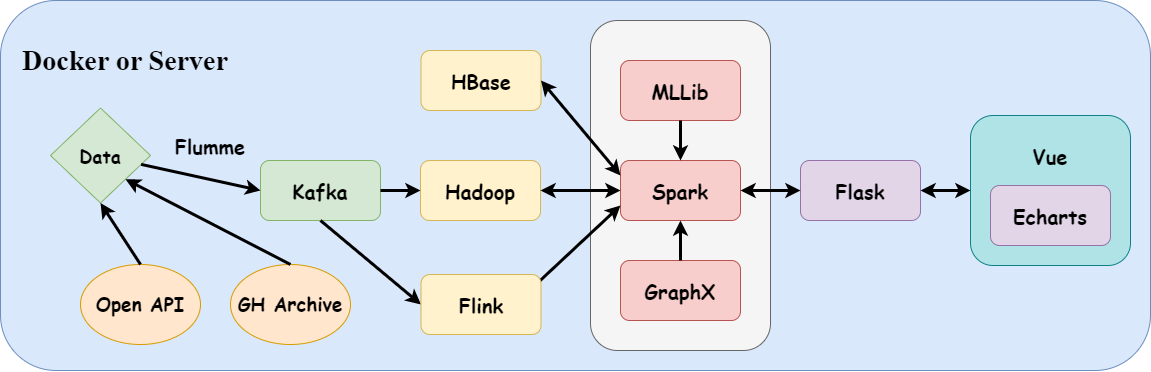
\includegraphics[width=0.53\textwidth]{./pic/dataflow.png}
        \caption{This picture show the rough technologies based on Dataflow.}
        \label{fig:dataflow}
    \end{figure}
% \end{strip}


\subsection{Big Data Process}

\begin{enumerate}
    \item \textbf{Spark}. As a computing engine, it will perform most of the data processing tasks.
    \item \textbf{Flumme} As a data collector, it will collect data from Github Archive and Github API.
    \item \textbf{Kafka}. As a message queue, it will simulate the real-time stream of Github Archive.
    \item \textbf{HDFS}. As a distributed file system, it will store the intermediate data as file or some persistant data.
    \item \textbf{Hive}. As a data warehouse, it will store the persistant data in tables.
    \item \textbf{Flink}. As a stream processing engine, it will process the real-time stream.
    \item \textbf{MLLib}. As a machine learning library, it will be used to extract features from data and finish some basic prediction tasks.
    \item \textbf{GraphX}. As a graph processing library, it will be used to construct a social graph.
    \item \textbf{HBase}. As a NoSQL database, it will be used to store some persistant data.
    \item \textbf{SparkNLP}. As a open-source library, it will perform the complicated NLP tasks. We will explore how to integrate it with Spark, because it's not an official library of Apache.
\end{enumerate}


\subsection{Data Visualization}

\begin{enumerate}
    \item \textbf{Vue}. As a front-end framework, it will be used to construct the basic framework of dashboard.
    \item \textbf{Echarts}. As a data visualization library, it will be used to visualize the results of data analysis.
\end{enumerate}

\subsection{Environment Deploy}

\begin{enumerate}
    \item \textbf{Docker}. Though the final application will be deployed on several cloud clusters. we may consider to deploy test environment on a powerful single machine locally by using Docker. By self-define images, it will help us construct the whole system easily and quickly.
    \item \textbf{Kubernetes}. As a container orchestration engine, it will be used to manage the containers. This will be used as a backup to set up the test system.
\end{enumerate}
